\section*{Задание}
В лабораторной работе анализируется результат выполнения трех программ. Программы демонстрируют открытие одного и того же файла несколько раз. Реализация, когда файл открывается в одной программе несколько раз выбрана для простоты. Однако, как правило, такая ситуация возможна в системе, когда один и тот же файл несколько раз открывают разные процессы или потоки одного процесса. При выполнении асинхронных процессов такая ситуация является вероятной и ее надо учитывать, чтобы избежать потери данных, получения неверного результата при выводе данных в файл или чтения данных не в той последовательности, в какой предполагалось, и в результате при обработке этих данных получения неверного результата.
Каждую из приведенных программ надо выполнить в многопоточном варианте: в программах создается дополнительный поток, а работа с открываемым файлом выполняется в потоках.

Проанализировать работу приведенных программ и объяснить результаты их работы.

\section*{struct \_IO\_FILE}
\begin{lstlisting}
struct _IO_FILE
{
int _flags;                /* High-order word is _IO_MAGIC; rest is flags. */

/* The following pointers correspond to the C++ streambuf protocol. */
char *_IO_read_ptr;        /* Current read pointer */
char *_IO_read_end;        /* End of get area. */
char *_IO_read_base;        /* Start of putback+get area. */
char *_IO_write_base;        /* Start of put area. */
char *_IO_write_ptr;        /* Current put pointer. */
char *_IO_write_end;        /* End of put area. */
char *_IO_buf_base;        /* Start of reserve area. */
char *_IO_buf_end;        /* End of reserve area. */

/* The following fields are used to support backing up and undo. */
char *_IO_save_base; /* Pointer to start of non-current get area. */
char *_IO_backup_base;  /* Pointer to first valid character of backup area */
char *_IO_save_end; /* Pointer to end of non-current get area. */

struct _IO_marker *_markers;

struct _IO_FILE *_chain;

int _fileno;
int _flags2;
__off_t _old_offset; /* This used to be _offset but it's too small.  */

/* 1+column number of pbase(); 0 is unknown. */
unsigned short _cur_column;
signed char _vtable_offset;
char _shortbuf[1];

_IO_lock_t *_lock;
#ifdef _IO_USE_OLD_IO_FILE
};

\end{lstlisting}

\section*{Программа №1}
\begin{lstinputlisting}[label=third,caption=Однопоточная версия, language=c, firstline=1, lastline=29]{../src/01_one_thread/main.c}
\end{lstinputlisting}

\subsection*{Результат работы}
\begin{figure}[H]
	\centering
	
\includegraphics[scale=0.5]{img/res_01_one.png}
	\caption{Однопоточная версия 1-ой программы}
	\label{fig:1}
\end{figure}

\begin{lstinputlisting}[label=third,caption=Многопоточная версия, language=c, firstline=1, lastline=32]{../src/01_two_threads/main.c}
\end{lstinputlisting}

\subsection*{Результат работы}
\begin{figure}[H]
	\centering
	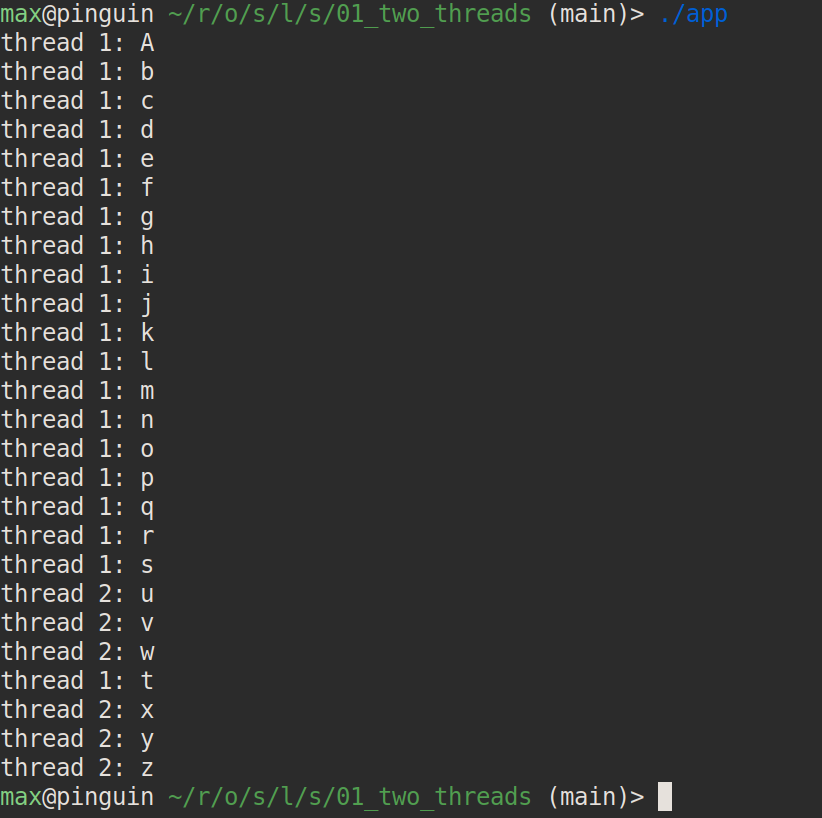
\includegraphics[scale=0.35]{img/res_01_two.png}
	\caption{Многопоточная версия 1-ой программы}
	\label{fig:2}
\end{figure}

\subsection*{Объяснение результатов}
\begin{figure}[H]
	\centering
	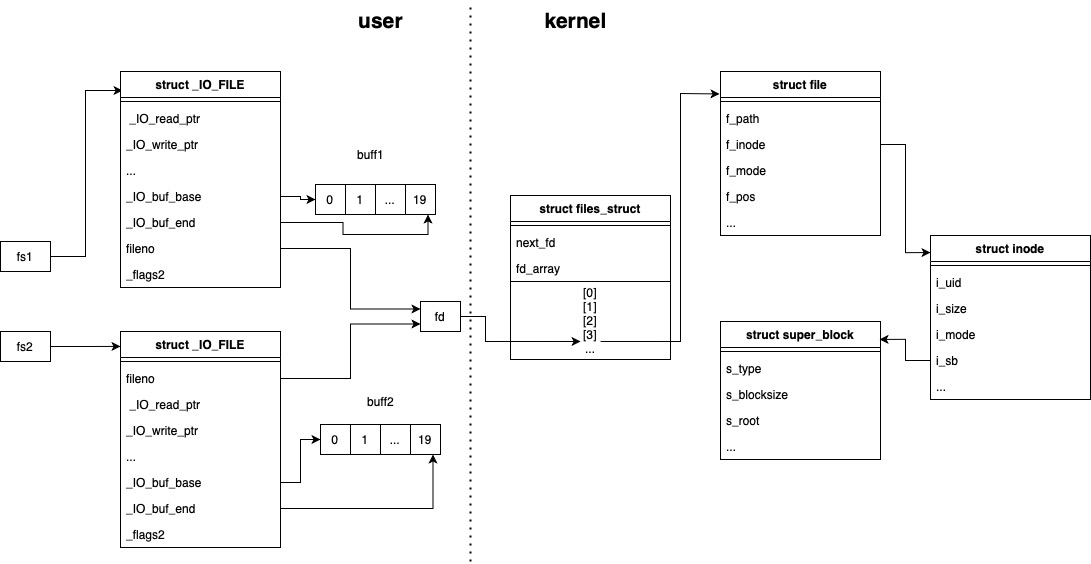
\includegraphics[scale=0.45]{img/os_lab_05-1.jpg}
	\caption{Связь структур}
	\label{fig:3}
\end{figure}
Работа с содержимым файла происходит через целочисленный файловый дескриптор, который представляет из себя номер строки в таблице ссылок на открытые файлы процесса. При помощи системного вызова open() создается файловый дескриптор fd, файл открывается на чтение, указатель на текущую позицию в файле устанавливается на начало файла. Если системный  вызов  завершается  успешно,  возвращенный  файловый  дескриптор является самым маленьким дескриптором, который еще не открыт  процессом. Возвращается -1 в случае ошибки. Функция fdopen связывает два потока на чтение с существующим файловым дескриптором fd. Функция setvbuf задает блочную буферизацию с размером буфера 20 байт. \underline{ }IOFBF - полная буферизация, то есть данные будут буферизироваться, пока буфер не заполниться полностью. В цикле данные считываются из двух потоков fs1 и fs2 в стандартный поток вывода stdout. Так как открытые файлы, для которых используется ввод/вывод потоков, буферизуются и размер буфера 20 байт, то в поток fs1 будут считаны первые 20 символов и указатель на текущую позицию в файле будет смещён на 20. В поток fs2 будут считаны оставшиеся 6 символов и символ конца строки.

\begin{itemize}
	\item в однопоточной версии вызовы fscanf(fs1, ...) и fscanf(fs2, ...) происходят поочерёдно, поэтому символы в результате соответствуют поочерёдному чтению из первого и второго буферов;
	\item в многопоточной версии порядок вызовов fscanf(fs, ...) двух потоков не определён, поэтому символы в результате соответствуют чтению из буферов в произвольном порядке.
\end{itemize}

\section*{Программа 2}
\begin{lstinputlisting}[label=third,caption=Однопоточная версия, language=c, firstline=1, lastline=24]{../src/02_one_thread/main.c}
\end{lstinputlisting}

\subsection*{Результат работы}
\begin{figure}[H]
	\centering
	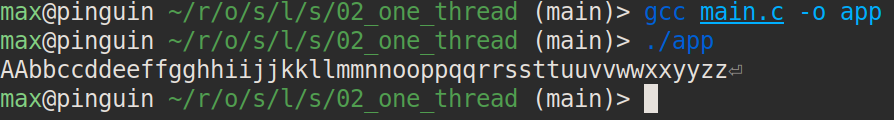
\includegraphics[scale=0.5]{img/res_02_one.png}
	\caption{Однопоточная версия 2-ой программы}
	\label{fig:4}
\end{figure}

\begin{lstinputlisting}[label=third,caption=Многопоточная версия, language=c, firstline=1, lastline=26]{../src/02_one_thread/main.c}
\end{lstinputlisting}

\subsection*{Результат работы}
\begin{figure}[H]
	\centering
	
\includegraphics[scale=0.5]{img/res_02_two.png}
	\caption{Многопоточная версия 2-ой программы}
	\label{fig:5}
\end{figure}

\subsection*{Объяснение результатов}
\begin{figure}[H]
	\centering
	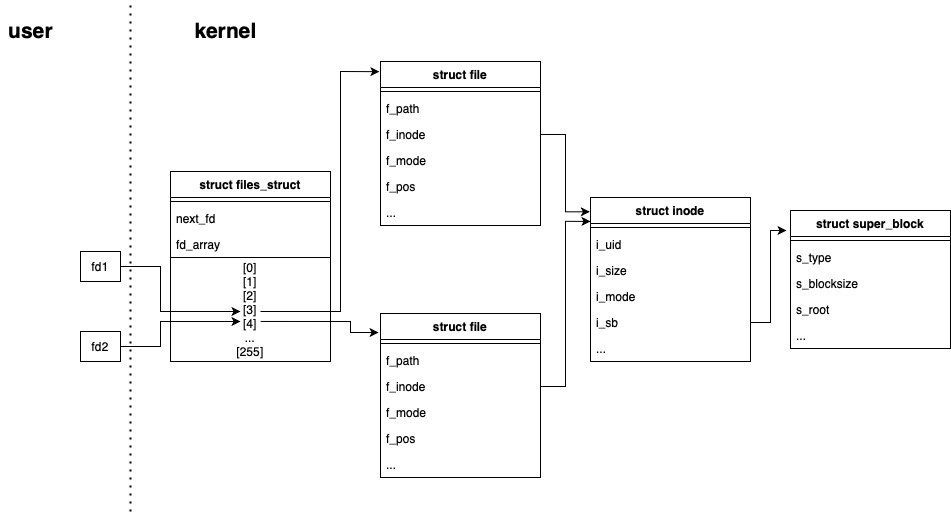
\includegraphics[scale=0.45]{img/os_lab_05-2.jpg}
	\caption{Связь структур}
	\label{fig:6}
\end{figure}
Системный вызов open() создаёт 2 файловых дескриптора открытого файла (описанного структурами struct file) и возвращает индекс в массиве fd\_array структуры files\_struct. Таким образом, создаётся две структуры открытого файла, каждая из которых имеет собственное поле f\_pos. Именно поэтому в результате будет получен приведённый результат:
\begin{itemize}
	\item в однопоточной версии вызовы read происходят поочерёдно, поэтому символы в результате соответствуют двум поочерёдным независимым чтениям из файла;
	\item в многопоточной версии порядок вызовов read двух потоков не определён, поэтому символы в результате соответствуют двум независимым чтениям в произвольном порядке.
\end{itemize}

\section*{Программа 3}
\begin{lstinputlisting}[label=third,caption=Программа 3, language=c, firstline=1, lastline=29]{../src/03_threads/main.c}
\end{lstinputlisting}

\subsection*{Результат работы}
\begin{figure}[H]
	\centering
	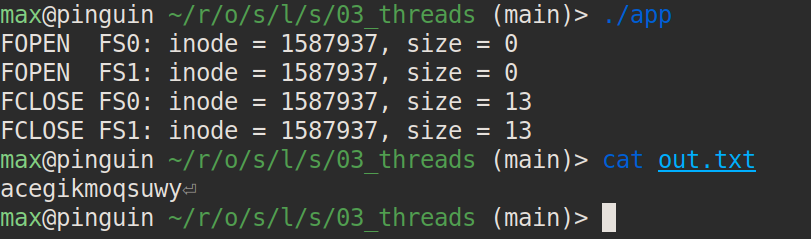
\includegraphics[scale=0.45]{img/res_03.png}
	\caption{3-я программа}
	\label{fig:1}
\end{figure}
\subsection*{Объяснение результатов}
\begin{figure}[H]
	\centering
	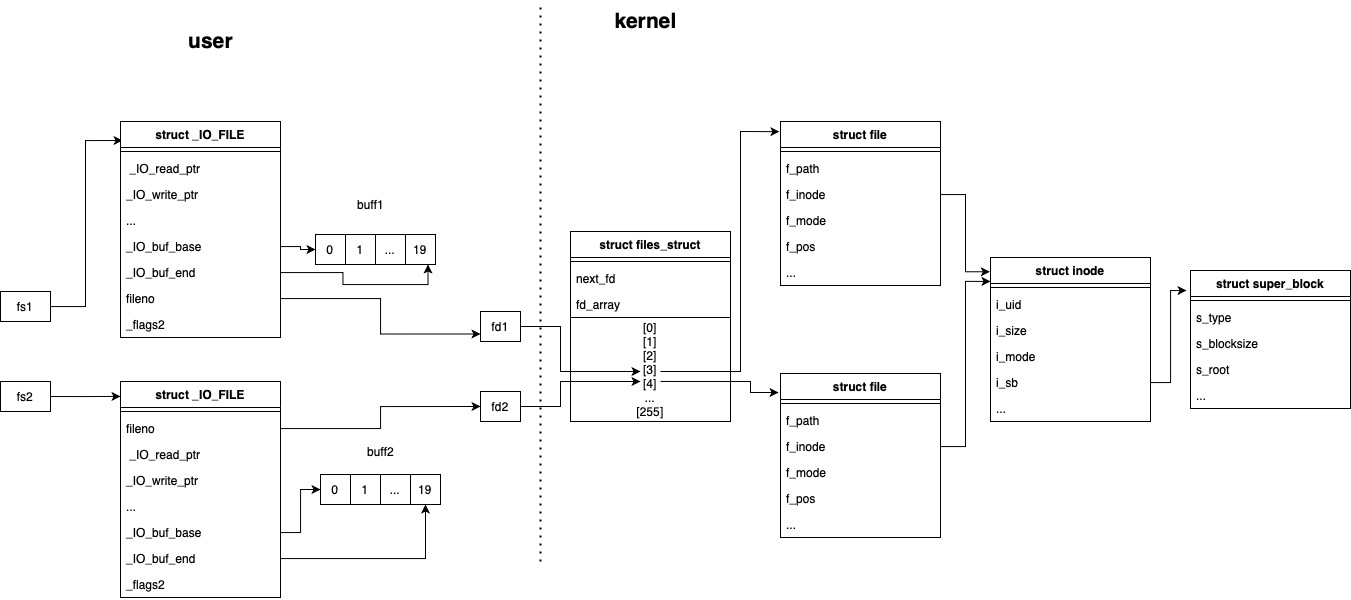
\includegraphics[scale=0.37]{img/os_lab_05-3.jpg}
	\caption{Связь структур}
	\label{fig:1}
\end{figure}
С помощью fopen() открываются два потока на запись, которые имеют разные файловые дескрипторы. Нечётные буквы алфавита записываются в первый поток, чётные - во второй. Так как функция fopen() выполняет ввод-вывод с буферизацией, окончательная запись в файл осуществляется либо при полном заполнении буфера, либо при вызове функций fclose() или функции fflush().

Так как запись производится с помощью функции fprintf, использующий буферизованный ввод-вывод, то запись в двух потоках будет осуществляться в буфер. Существуют 3 условия записи из буфера в файл:
\begin{itemize}
	\item переполнение буфера;
	\item fflush;
	\item закрытие файла.
\end{itemize}

Так как буфер не переполняется и не вызывается fflush, то запись в файл в приведённой программе осуществится лишь при вызове fclose. Так как потоки работают с одним и тем же файлом, причём ссылаются на разные структуры struct file (то есть поле f\_pos для каждого потока своё), то результат записи будет зависеть от того, какой поток вызвал fclose позже. При этом данные, записанные в файл ранее, будут утеряны.

\subsection*{Решение проблемы}
Причина: каждый дескриптор открытого файла имеет своё поле f\_pos. 

\textbf{Решение №1}: необходимо использовать режим O\_APPEND. В данном режиме перемещение позиции в конец файла и добавление символа происходят атомарно, поэтому данные не будут утеряны. 

\textbf{Решение №2}: необходимо использовать мьютекс для перемещения позиции в конец файла и записи символа. Код:
\begin{lstinputlisting}[label=third,caption=Решение с мьютексом, language=c, firstline=1, lastline=41]{../src/03_threads/solved_2/main.c}
\end{lstinputlisting}